\documentclass[tikz,border=10pt]{standalone}
\usetikzlibrary{arrows.meta,positioning}
\usepackage{mathtools}

\begin{document}
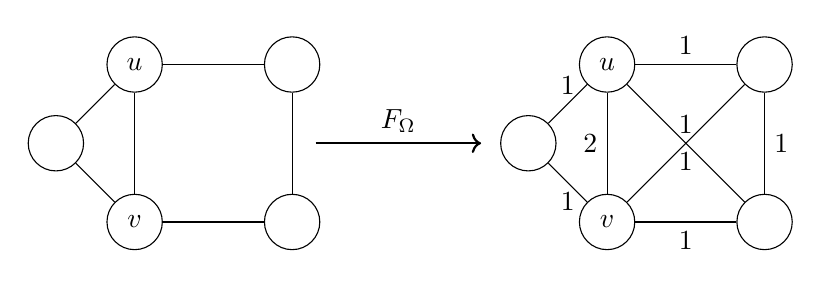
\begin{tikzpicture}[vertex/.style={circle,draw,minimum size=2em,inner sep=3pt}, edge/.style={-}]
  % Vertices
  \node[vertex] (y) at (-1,1) {$\,$};
  \node[vertex] (u) at (0,2) {$u$};
  \node[vertex] (v) at (0,0) {$v$};
  \node[vertex] (w) at (2,0) {$\,$};
  \node[vertex] (x) at (2,2) {$\,$};
  
  % Edges
  \draw[edge] (y) -- (u);
  \draw[edge] (y) -- (v);
  \draw[edge] (u) -- (v);
  \draw[edge] (v) -- (w);
  \draw[edge] (w) -- (x);
  \draw[edge] (x) -- (u);

  % Transformed vertices
  \node[vertex] (y2) at (5,1) {$\,$};
  \node[vertex] (u2) at (6,2) {$u$};
  \node[vertex] (v2) at (6,0) {$v$};
  \node[vertex] (w2) at (8,0) {$\,$};
  \node[vertex] (x2) at (8,2) {$\,$};
  
  % Transformed edges
  \draw[edge] (u2) -- node[above] {1} (x2);
  \draw[edge] (x2) -- node[right] {1} (w2);
  \draw[edge] (w2) -- node[below] {1} (v2);
  \draw[edge] (v2) -- node[left] {2} (u2);
  \draw[edge] (u2) -- node[above] {1} (w2);
  \draw[edge] (v2) -- node[below] {1} (x2);
  \draw[edge] (y2) -- node[above] {1} (u2);
  \draw[edge] (y2) -- node[below] {1} (v2);

  % Transformation arrow
  \draw[->,thick] (2.3,1) -- (4.4,1) node [pos=0.5,above] {$F_\Omega$};
\end{tikzpicture}
\end{document}